%
\comment{

1. OpenFlow uses the multiple match table (MMT) model
2. The MMT model has limitations
3. Some recent work addresses these limitations: one building some programmability into ASICs, the other building in an FPGA

}
%

\begin{figure}
\centering
%
        \begin{subfigure}[t]{0.5\textwidth}
        		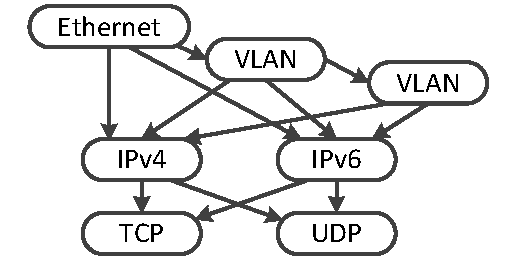
\includegraphics[width=\textwidth]{figs/parse-graph.pdf}
        		\caption{Parse Graph}
        		\label{parse-graph}
		\end{subfigure}
        \begin{subfigure}[t]{0.5\textwidth}
        		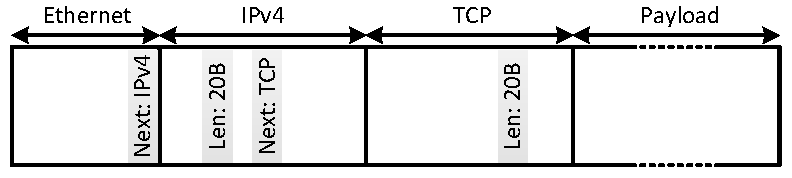
\includegraphics[width=\textwidth]{figs/packet.pdf}
        		\caption{TCP/IP Packet}
        		\label{packet}
		\end{subfigure}
\caption{An example parse graph commonly seen in enterprise networks, and a packet belonging to that parse graph. A parse graph can be used to represent the combinations of protocols that a packet processor may see in a certain application.}
\label{parse-graph-packet}
\end{figure}
%

Depending on the application, a packet processor must be able to process packets of a certain set of protocols.
These protocols vary depending on the type of packet and layer they represent on the OSI stack.
For example, Ethernet is one of the most common layer 2 protocols found in modern networks.
The protocol at each layer contains information regarding the type and location of the protocol found in the next higher layer (Figure~\ref{packet}).
The various different combinations of protocols that may be received in a single packet can be represented by a parsing graph~\cite{gibb2013design} (Figure~\ref{parse-graph}).

As network protocols are changed, added and replaced, a programmable packet processor must be able to be reconfigured to support different parsing graphs.
%OpenFlow-based processors use match tables to traverse these graphs.
The OpenFlow standard comes with specifications for architecting an SDN-compatible packet processor~\cite{opennet}.
The architecture is based on a cascade of match-action ``flow'' tables: memory holding all possible values of relevant packet header fields, and instructions for what action to be taken once matched.
Figure~\ref{openflow-pp} illustrates the high level design of this architecture.
The pipeline begins by matching fields whose locations in the packet header are known.
%When a field is matched at a table entry for a protocol at a certain OSI stack layer, the entry contains information regarding where to look in the next match table for the protocol of the next layer.
When a field is matched, the entry contains information regarding where to look in the next match table for the protocol of the next layer, as well as any other corresponding actions to be taken.
This model requires match tables to contain all possible combinations of header protocols and field values that the processor may face.
All of the tables in the pipeline are populated by the control plane, such that lookups in a Table \textit{j} can depend on information from any Table \textit{i} so long as \textit{i} $<$ \textit{j}.

%The OpenFlow standard comes with specifications for architecting an SDN-compatible packet processor~\cite{opennet}.
%The architecture is based on a cascade of match-action ``flow'' tables: memory holding all possible values of relevant packet header fields, and instructions for what action to be taken once matched.
%Figure~\ref{openflow-pp} illustrates the high level design of this architecture.
%The pipeline begins by matching fields whose locations in the packet header are known, and determining corresponding actions to take based on what values are matched.
%Information from these matches can then be used to determine the location of other packet header fields to perform matching in later stages of the pipeline.
%All of the tables in the pipeline are populated by the control plane, such that lookups in a Table \textit{j} can depend on information from any Table \textit{i} so long as \textit{i} $<$ \textit{j}.

There are two important limitations to this programmable packet processor design.
When built in an ASIC, the number of tables along with their width and depth are fixed upon chip fabrication.
Consequently, should a new protocol be created that requires fields that are larger than the table width, a number of entries that exceeds the table depth, or more pipeline stages than are available, then the packet processor can not be configured to support such a protocol.
Similarly, the action set available is also set upon fabrication.
Any new actions required by newly developed protocols could not be supported.

%
%
%


Recent work has revealed two possible ways to address these limitations.
Bosshart \textit{et al.} proposed building in additional programmability into an ASIC-based packet processor through the use of ternary content-addressable memory (TCAMs)~\cite{bosshart2013forwarding}.
Their design -- called RMT (Reconfigurable Match Tables) -- can be viewed as an upgrade to the OpenFlow model.
It involves mapping logical match (or flow) tables to physical ones by allowing a logical table to use resources from multiple pipeline stages.
This mapping process allows the width and depth of flow tables to be customized for specific sets of protocols.
Additionally, their design implements a reduced instruction set that, when used in combinations in a very-long instruction word, can execute a wider array of actions than OpenFlow.

The RMT design mitigates, but does not solve OpenFlow's limitations.
As the authors admit in the paper, their design is still restricted by the number of pipeline stages, table sizes, and action units made available to the chip upon fabrication.
These restrictions cannot be avoided when building a programmable packet processor from ASIC technology.
In contrast, Attig and Brebner have previously shown that a programmable packet parser can be built on an FPGA that supports 400 Gb/s bandwidth~\cite{attig2011400}.
Their design -- which they refer to as PP\footnote{Attig and Brebner use ``PP'' to refer to the language used to program their architecture. For simplicity, we shall use PP to refer to their design as a whole.} -- still uses a sequence of match tables, with each match stage determining the location of fields to be matched in the next stage.
Using an FPGA allows their design to be reconfigured in the field to support different table configurations and actions.

Our programmable packet processor design also leverages FPGA technology to avoid the limited flexibility of ASIC-based designs.
However, unlike the PP design, we elect to avoid using the recommended OpenFlow architecture, which was originally proposed to bring programmability to ASIC-based network infrastructures.
We instead embrace the full reconfigurability of the FPGA, creating a fully-programmable packet processor that is more efficient than the FPGA-based PP design and more flexible than the ASIC-based RMT design.

\figvs{1}{openflow-pp}{}{High-level overview of OpenFlow's programmable packet processor architecture~\cite{opennet}.}
